\chapter{Machine Learning}

	\section{\texttt{NNClass}: Simple neural network classifier module}

	A simple bit of code for training classification neural networks.
	
	\subsection{Installation}
	
	Install from \texttt{pip3}:
	
	\begin{minted}{bash}
	pip3 install --user NNClass
	\end{minted}
	
	Or by cloning this repository:
	
	\begin{minted}{bash}
	#clone the repo
	git clone https://github.com/mattkjames7/NNClass
	cd NNClass
	
	#Either create a wheel and use pip: (X.X.X should be replaced with the current version)
	python3 setup.py bdist_wheel
	pip3 install --user dists/NNClass-X.X.X-py3-none-any.whl
	
	#Or by using setup.py directly
	python3 setup.py install --user
	\end{minted}
	
	
	\subsection{Usage}
	
	Start by training a network:
	
	\begin{minted}{python}
	import NNClass as nnc
	
	#create the network, defining the activation functions and the number of nodes in each layer
	net = nnc.NNClass(s,AF='sigmoid',Output='softmax')
	
	#note that s should be a list, where each element denotes the number of nodes in each layer
	
	#input training data
	net.AddData(X,y)
	#Input matrix X should be of the shape (m,n) - where m is the number of samples and n is the number of input features
	#Output hypothesis matrix y should either be
	# an array (m,) of integers corresponding to class
	# or matrix (m,k) of one-hot labels
	
	#optionally add validation and test data
	net.AddValidationData(Xv,yv)
	#Note that validation data is ignored if kfolds > 1 during training
	net.AddTestData(Xt,yt)
	
	#Train the network 
	net.Train(nEpoch,kfolds=k)
	#nEpoch is the number of training epochs
	#kfolds is the number of kfolds to do - if kfolds > 1 then the training data are split 
	#into kfold sets, each of which has a turn at being the validation set. This results in
	#kfold networks being trained in total (net.model)
	#see docstring net.Train? to see more options
	\end{minted}
	
	After training, the cost function may be plotted:
	
	\begin{minted}{python}
	net.PlotCost(k=k)
	\end{minted}
	
	We can use the network on other data:
	
	\begin{minted}{python}
	#X in this case is a new matrix
	y = net.Predict(X)
	\end{minted}
	
	The networks can be saved and reloaded:
	
	\begin{minted}{python}
	#save
	net.Save(fname='networkname.bin')
	
	#reload
	net = nnc.LoadANN(fname='networkname.bin')
	\end{minted}
	
	Running \mintinline{python}{mnist = nnc.Test()} will perform a test on the code, by training a neural network to classify a set of hand-written digits (0-9) from the MNIST dataset (https://deepai.org/dataset/mnist). The function will then plot out the cost, accuracy and an example of a classified digit, e.g.:
	
	\begin{figure}[H]
	  \centering
	  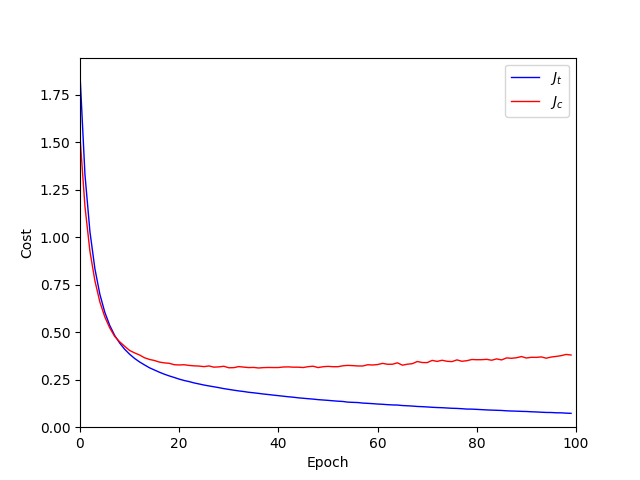
\includegraphics[width=0.7\textwidth]{figures/ch6_nnccost.png}
	  \caption{Cost plot}
	\end{figure}
	
	\begin{figure}[H]
	  \centering
	  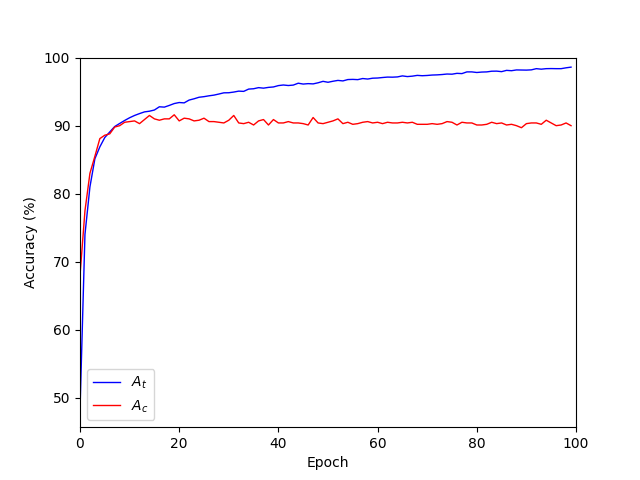
\includegraphics[width=0.7\textwidth]{figures/ch6_nncaccuracy.png}
	  \caption{Accuracy plot}
	\end{figure}
	
	\begin{figure}[H]
	  \centering
	  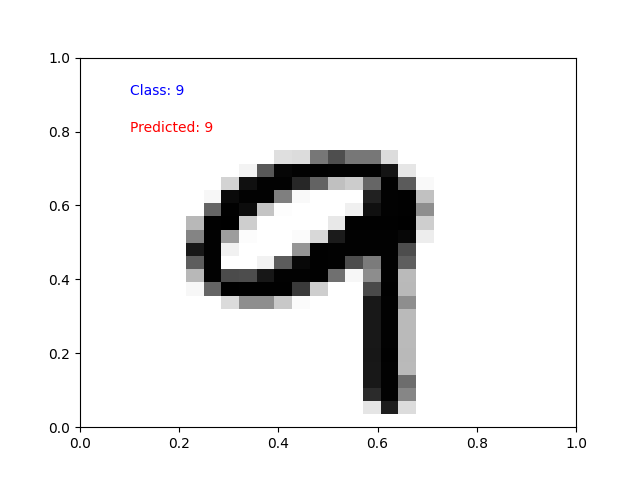
\includegraphics[width=0.5\textwidth]{figures/ch6_nncdigit.png}
	  \caption{Example of a classified digit}
	\end{figure}
	
	The 10,000 sample MNIST data can be accessed using the \texttt{NNClass.MNIST} object.
	

	\section{\texttt{NNFunction}: Train neural networks on arbitrary functions}

	A simple package for modelling multidimensional non-linear functions using artificial neural networks.

	\subsection{Installation}
	
	Install from \texttt{pip3}:
	
	\begin{minted}{bash}
	pip3 install --user NNFunction
	\end{minted}
	
	Or by cloning this repository:
	
	\begin{minted}{bash}
	#clone the repo
	git clone https://github.com/mattkjames7/NNFunction
	cd NNFunction
	
	#Either create a wheel and use pip: (X.X.X should be replaced with the current version)
	python3 setup.py bdist_wheel
	pip3 install --user dists/NNFunction-X.X.X-py3-none-any.whl
	
	#Or by using setup.py directly
	python3 setup.py install --user
	\end{minted}
	
	
	\subsection{Usage}
	
	Start by training a network:
	
	\begin{minted}{python}
	import NNFunction as nnf
	
	#create the network, defining the activation functions and the number of nodes in each layer
	net = nnf.NNFunction(s,AF='softplus',Output='linear')
	
	#note that s should be a list, where each element denotes the number of nodes in each layer
	
	#input training data
	net.AddData(X,y)
	#Input matrix X should be of the shape (m,n) - where m is the number of samples and n is the number of input features
	#Output hypothesis matrix y should have the shape (m,k) - where k is the number of output nodes
	
	#optionally add validation and test data
	net.AddValidationData(Xv,yv)
	#Note that validation data is ignored if kfolds > 1 during training
	net.AddTestData(Xt,yt)
	
	#Train the network 
	net.Train(nEpoch,kfolds=k)
	#nEpoch is the number of training epochs
	#kfolds is the number of kfolds to do - if kfolds > 1 then the training data are split 
	#into kfold sets, each of which has a turn at being the validation set. This results in
	#kfold networks being trained in total (net.model)
	#see docstring net.Train? to see more options
	\end{minted}
	
	After training, the cost function may be plotted:
	
	\begin{minted}{python}
	net.PlotCost(k=k)
	\end{minted}
	
	We can use the network on other data:
	
	\begin{minted}{python}
	#X in this case is a new matrix
	y = net.Predict(X)
	\end{minted}
	
	The networks can be saved and reloaded:
	
	\begin{minted}{python}
	#save
	net.Save(fname='networkname.bin')
	
	#reload
	net = nnf.LoadANN(fname='networkname.bin')
	\end{minted}
	
	The animation below demonstrates the training of a neural network used to reproduce four different functions simultaneously. It was produced using \texttt{NNFunction.TrainNN4}.
	
	\begin{figure}[H]
	  \centering
	  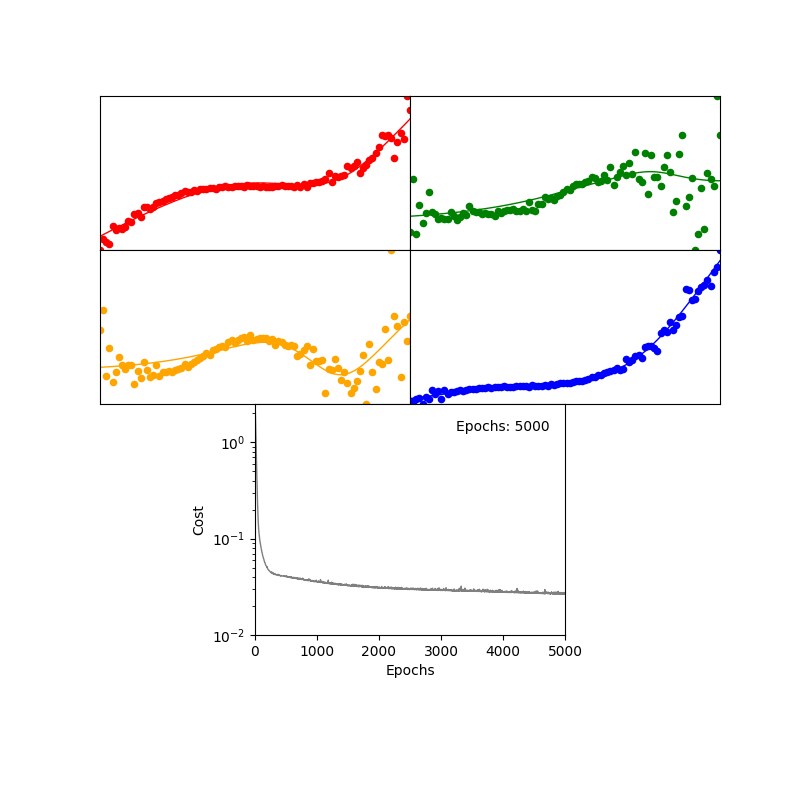
\includegraphics[width=\textwidth]{figures/ch6_nnfunc.gif}
	\end{figure}


	%\section{\texttt{PyNeuralNetwork}: Crap neural network code}

	%\section{\texttt{fipsnn}: The neural networks used to classify FIPS data}

	%\section{\texttt{pydataclust}: Python module for clustering data}